%%%
\begin{frame}[fragile]{\tbf{Internship - M1} \\ 
\small{ElastoHydroDynamics interactions \& Modified fluctuation-dissipation relation}}

\tbf{Equations of motion (EOM) are non-linearly coupled}  
\ \\

%%%
\begin{minipage}{0.36\linewidth}
\begin{center}
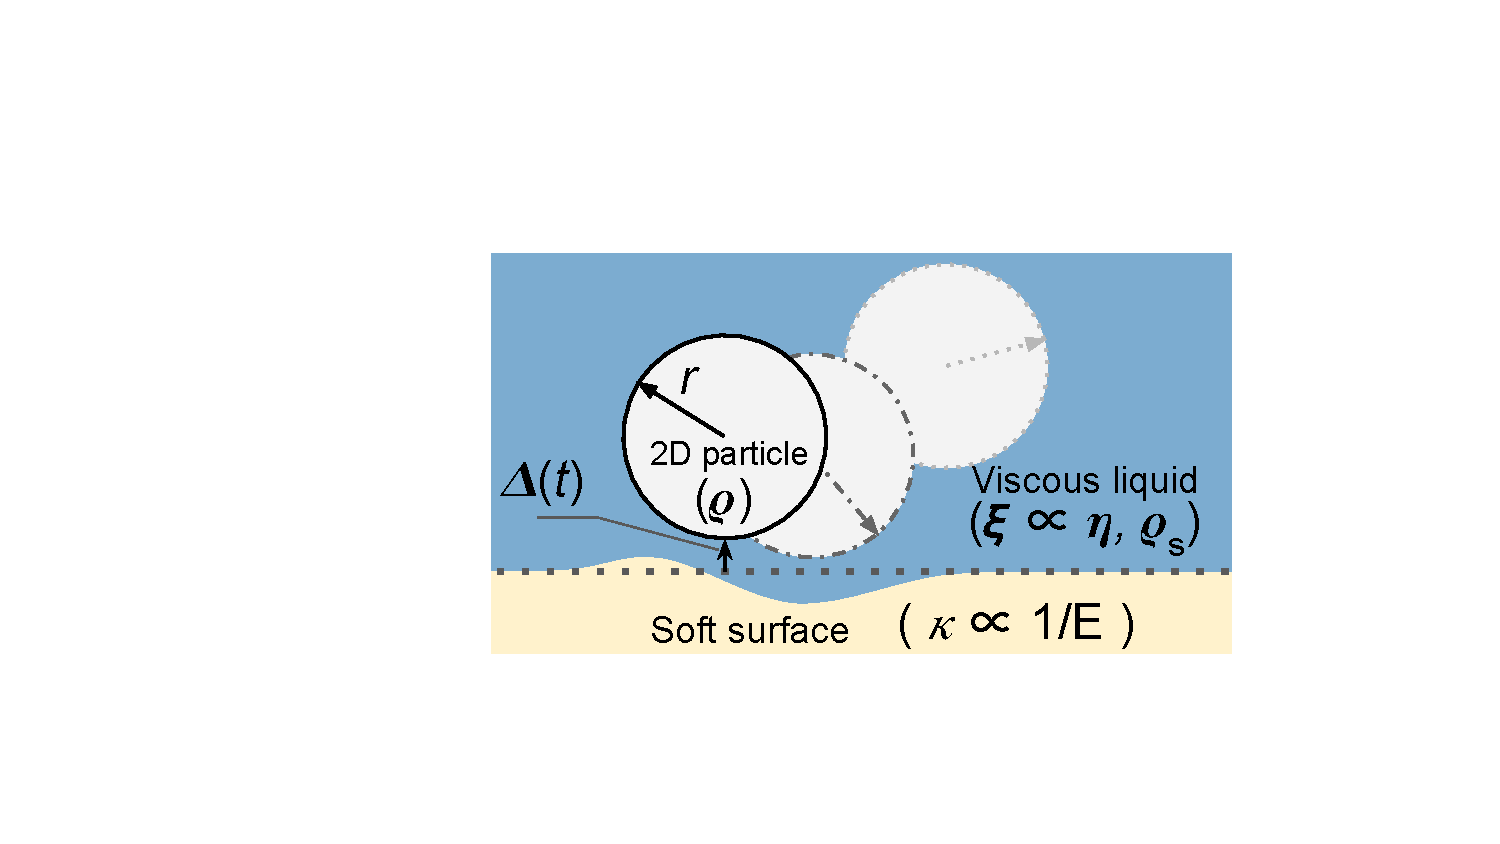
\includegraphics[height=2.2cm]{figs/BEHD_JPS.pdf}
\end{center}
\end{minipage}
%%%
\begin{minipage}{0.58\linewidth}
\footnotesize
$$ \agn{
\textcolor{red}{\ddot{X}_\mrm{G}} + \frac{2\textcolor{black}{\veps} \textcolor{cyan}{\xi}}{3} \frac{\blendcolors*{!60}\textcolor{red}{\dot{X}_\mrm{G}}}{\sqrt{{\blendcolors*{!60}\textcolor{orange}{\Delta}}}} + \frac{\textcolor{violet}{\kappa} \textcolor{black}{\veps} \textcolor{cyan}{\xi}}{6} \left[ \frac{19}{4} \frac{\dot{\blendcolors*{!60}\textcolor{orange}{\Delta}} \blendcolors*{!60}\textcolor{red}{\dot{X}_\mrm{G}}}{{\blendcolors*{!60}\textcolor{orange}{\Delta}}^{7/2}} - \frac{\dot{\blendcolors*{!60}\textcolor{orange}{\Delta}} \dot{\blendcolors*{!60}\textcolor{blue}{\Theta}}}{{\blendcolors*{!60}\textcolor{orange}{\Delta}}^{7/2}} + \frac{1}{2} \frac{\textcolor{blue}{\ddot{\blendcolors*{!60}\textcolor{blue}{\Theta}}} - \textcolor{red}{\ddot{X}_\mrm{G}}}{{\blendcolors*{!60}\textcolor{orange}{\Delta}}^{5/2}} \right] &= 0 \\
%\ddot{{\textcolor{orange}{\Delta}}} + \textcolor{cyan}{\xi} \frac{\dot{{\blendcolors*{!60}\textcolor{orange}{\Delta}}}}{{\blendcolors*{!60}\textcolor{orange}{\Delta}}^{3/2}} + \frac{\textcolor{violet}{\kappa} \textcolor{cyan}{\xi}}{4} \left[ 21 \frac{\dot{{\blendcolors*{!60}\textcolor{orange}{\Delta}}}^2}{{\blendcolors*{!60}\textcolor{orange}{\Delta}}^{9/2}} - \frac{(\dot{\blendcolors*{!60}\textcolor{blue}{\Theta}} - \blendcolors*{!60}\textcolor{red}{\dot{X}_\mrm{G}})^2}{{\blendcolors*{!60}\textcolor{orange}{\Delta}}^{7/2}} - \frac{15}{2} \frac{\ddot{{\textcolor{orange}{\Delta}}}}{{\blendcolors*{!60}\textcolor{orange}{\Delta}}^{7/2}} \right] &= 0 \\
%\textcolor{blue}{\ddot{\Theta}} + \frac{4\textcolor{black}{\veps}\textcolor{cyan}{\xi}}{3} \frac{\dot{\blendcolors*{!60}\textcolor{blue}{\Theta}}}{\sqrt{{\blendcolors*{!60}\textcolor{orange}{\Delta}}}} + \frac{\textcolor{violet}{\kappa} \textcolor{black}{\veps} \textcolor{cyan}{\xi}}{3} \left[ \frac{19}{4} \frac{\dot{\blendcolors*{!60}\textcolor{orange}{\Delta}} \dot{\blendcolors*{!60}\textcolor{blue}{\Theta}}}{{\blendcolors*{!60}\textcolor{orange}{\Delta}}^{7/2}} - \frac{\dot{\blendcolors*{!60}\textcolor{orange}{\Delta}} \blendcolors*{!60}\textcolor{red}{\dot{X}_\mrm{G}}}{{\blendcolors*{!60}\textcolor{orange}{\Delta}}^{7/2}} + \frac{1}{2} \frac{\textcolor{red}{\ddot{X}_\mrm{G}} - \textcolor{blue}{\ddot{\Theta}}}{{\blendcolors*{!60}\textcolor{orange}{\Delta}}^{5/2}} \right] &= 0 
\dot{v} + f({\blendcolors*{!60}\textcolor{orange}{\Delta}}) \ v + \textcolor{violet}{\kappa} \ g(\dot{v},v,{\blendcolors*{!60}\textcolor{orange}{\Delta}}) = 0 
\fives \to \fives
\dot{v} = - \gamma_{\mathrm{eff}} \  v +& \textcolor{}{\dlt F}/ M \\
  \lla \dlt F_i^2 \rra \propto \frac{2 m_i \gma_{i\textcolor{blue}{0}}}{\beta} \lls 1 - \textcolor{violet}{\kappa} \cdot \frac{\gma_{i\textcolor{red}{1}} ({\blendcolors*{!90}\textcolor{orange}{\Delta}}) }{\gma_{i\textcolor{blue}{0}} ({\blendcolors*{!90}\textcolor{orange}{\Delta}})} \rrs  
\fives
\frac{D(\textcolor{violet}{\kappa}, {\blendcolors*{!90}\textcolor{orange}{\Delta}})}{D(\textcolor{violet}{0}, {\blendcolors*{!90}\textcolor{orange}{\Delta}})}  =  1 -& \textcolor{violet}{\kappa} \cdot \frac{\gma_{i\textcolor{red}{1}} ({\blendcolors*{!90}\textcolor{orange}{\Delta}}) }{\gma_{i\textcolor{blue}{0}} ({\blendcolors*{!90}\textcolor{orange}{\Delta}}) }
} $$
\end{minipage}
\bigskip

\footnotesize{T. Salez, and L. Mahadevan, \tit{J. Fluid Mech.} \tbf{2015}, \tit{779}, 181-196}


\ \\ \pause


\normalsize
\tbf{Add random force into EOM for \uwave{modified fluctuation-dissipation relation}}


\begin{comment}

%%%
\begin{minipage}{0.5\linewidth}



\small
\begin{center}
\begin{tikzpicture}[node distance=10pt]
  \node[] (vadd) {$v_i = v_{i\textcolor{blue}{0}} + \textcolor{violet}{\kappa} \cdot v_{i\textcolor{red}{1}}$};
  \node[, right=of vadd] (vcrr) {$\lla v_{i\textcolor{blue}{0}} v_{i\textcolor{red}{1}} \rra (t,\textcolor{violet}{\kappa})$};
  \node[, below=1pt of vcrr] (gma) {$\gma_{i} = \gma_{i\textcolor{blue}{0}} ({\blendcolors*{!90}\textcolor{orange}{\Delta}}) + \textcolor{violet}{\kappa} \cdot \gma_{i\textcolor{red}{1}} ({\blendcolors*{!90}\textcolor{orange}{\Delta}})$}; % draw -> \boxed{}
  \node[, below=1pt of gma] (fcrr) {$\lla \delta F_{i\textcolor{blue}{0}} \delta F_{i\textcolor{red}{1}} \rra (\textcolor{violet}{\kappa})$};
  \node[, left=of fcrr] (fadd) {$\delta F_i = \delta F_{i\textcolor{blue}{0}} + \textcolor{violet}{\kappa} \cdot \delta F_{i\textcolor{red}{1}}$};
  \node[text width=1cm, align=center, right=10 pt of gma] (noise) {noise-correlator \\ amplitude }  
  
  \draw[->] (vadd)  -- (vcrr);
  \draw[->] (fadd) -- (fcrr);
  \draw[->] (vcrr) -- (noise);
  \draw[->] (fcrr) -- (noise);
  \draw[->] (gma) -- (noise);
\end{tikzpicture}
\end{center}



%\normalsize
\small
$$  \lla \dlt F_i^2 \rra \propto \frac{2 m_i \gma_{i\textcolor{blue}{0}}}{\beta} \lls 1 - \textcolor{violet}{\kappa} \cdot \frac{\gma_{i\textcolor{red}{1}} ({\blendcolors*{!90}\textcolor{orange}{\Delta}}) }{\gma_{i\textcolor{blue}{0}} ({\blendcolors*{!90}\textcolor{orange}{\Delta}})} \rrs  $$

$$ D(\textcolor{violet}{\kappa}, {\blendcolors*{!90}\textcolor{orange}{\Delta}}) = D(\textcolor{violet}{0}, {\blendcolors*{!90}\textcolor{orange}{\Delta}}) \lls 1 - \textcolor{violet}{\kappa} \cdot \frac{\gma_{i\textcolor{red}{1}} ({\blendcolors*{!90}\textcolor{orange}{\Delta}}) }{\gma_{i\textcolor{blue}{0}} ({\blendcolors*{!90}\textcolor{orange}{\Delta}}) } \rrs $$


\end{minipage}
%%%
\begin{minipage}{0.01\linewidth}
\end{minipage}
%%%
\begin{minipage}{0.48\linewidth}
\begin{center}
%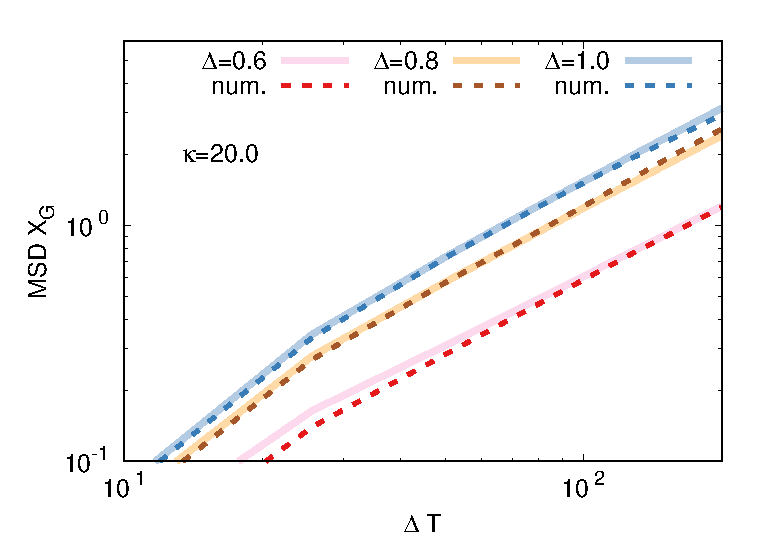
\includegraphics[height=3.0cm]{figs/msd_x-k20-2.eps}
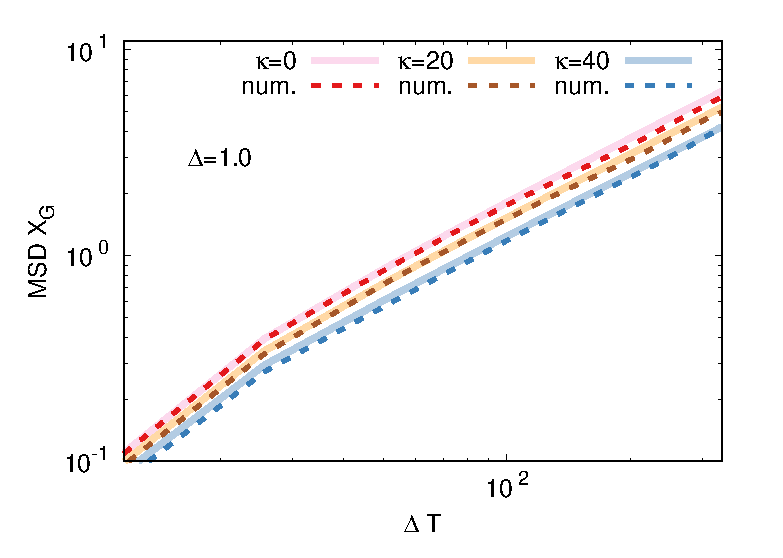
\includegraphics[height=4.0cm]{figs/msd_x-d1k2.eps}
\end{center}
\end{minipage}



\end{comment}
%\ \\

%\ \\


%%%
\begin{minipage}{0.45\linewidth}
\begin{center}
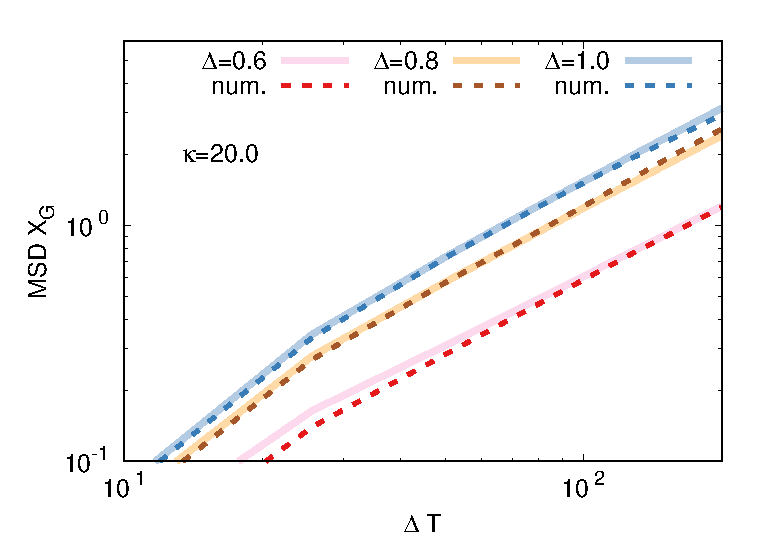
\includegraphics[height=3.7cm]{figs/msd_x-k20-2.eps}
\end{center}
\end{minipage}
%%%
\begin{minipage}{0.05\linewidth}
	\ \\
\end{minipage}
%%%
\begin{minipage}{0.45\linewidth}
\begin{center}
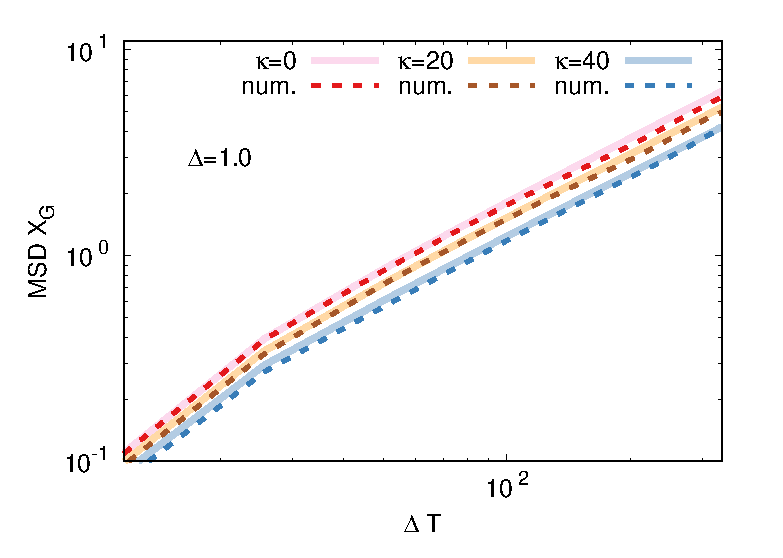
\includegraphics[height=3.7cm]{figs/msd_x-d1k2.eps}
\end{center}
\end{minipage}



\end{frame}
